\documentclass[12pt, a4paper]{article}
\usepackage[spanish]{babel}
%\usepackage{a4wide}
\usepackage{amsmath}
\usepackage{amssymb}
\usepackage{amsthm}
\usepackage{color}
\usepackage{hyperref}
\usepackage{makeidx}
\usepackage{float}
\usepackage[margin=1.0in]{geometry}
\usepackage{caratula}
\usepackage{pdfpages}

\usepackage{listings}\usepackage{color}
\usepackage{textcomp}\definecolor{listinggray}{gray}{0.9}

\definecolor{lbcolor}{rgb}{0.9,0.9,0.9}
\usepackage{a4wide}

\lstset{
      language=C++,
      basicstyle=\small\sffamily,
      columns=fullflexible,
      upquote=true,
      extendedchars=true,
      texcl=true,
      mathescape=true,
      showspaces=false
                }
            


\makeindex

\begin{document}

\index{Caratula}
%Estos son los parametros para la caratula
\materia{M\'etodos Num\'ericos}
\submateria{Recuperatorio Trabajo Pr\'actico 2}
\titulo{Filtrado de se\~nales usando DCT}
\fecha{19 de Julio de 2013}
\integrante{Zajdband, Dan}{144/10}{dan.zajdband@gmail.com}
\integrante{Ferreria, Manuel}{199/10}{m.ferreria@gmail.com}
\integrante{Taravilse, Leopoldo}{464/08}{ltaravilse@gmail.com}
\resumen{Estudio comparativo de filtros de se\~nales mediante la utilizaci\'on
de la DCT. An\'alisis del efecto de diversos filtros para distintos casos de
ruido (Senoidal y Blanco). Extensi\'on del problema a dos dimensiones. Estudio
del error de recuperaci\'on de la se\~nal original mediante la utilizaci\'on del
PSNR.}
\kwagregar{DCT, FFT, Fourier, Noise Reduction, Image analysis}

\maketitle

\pagebreak

\tableofcontents

\pagebreak

\index{Introducci\'on te\'orica}
\section{Introducci\'on te\'orica}

Previo al detalle del experimento realizado se detallan una serie de conceptos te\'oricos de necesario
conocimeinto para el entendimiento del trabajo.

\subsection{Reconocimiento \'optico de caracteres (OCR)}

El reconocimiento \'optico de caracteres es el proceso de conversi\'on de caracteres de un formato que puede
ser escritura a mano alzada, im\'agenes de libros u otros formatos complejos de entender para una computadora
a otro que sea reconocible por esta.

Este area combina disciplinas como inteligencia articifial, an\'alisis num\'erico y machine learning. Entre
las aplicaciones de OCR se encuentran:

\begin{itemize}
  \item Digitalizaci\'on de libros y documentos
  \item Reconocimiento de tarjetas de cr\'edito y facturas
  \item Generaci\'on de im\'agenes a partir de documentos digitales
  \item Resoluci\'on autom\'atica de CAPTCHA
\end{itemize}

\subsection{Matriz de covarianza}

Dado un conjunto de datos de $n$ componentes, se define la matriz de covarianza a la matriz de $n*n$ que
contiene en su elemento $(i, j)$ la covarianza entre las componentes $i$ y $j$ de la matriz original.

Siendo la covarianza entre 2 componentes definida como:

$\Sigma_{ij} = \mathrm{cov}(X_i, X_j) = \mathrm{E}\begin{bmatrix} (X_i - \mu_i)(X_j - \mu_j) \end{bmatrix}$

con $\mu_i = \mathrm{E}(X_i)$.

\subsection{Descomposici\'on en valores singulares (SVD)}

La descomposici\'on en valores singulares de una matriz $\mathbf{M} \in \mathbb{R}^{m \times n}$ es una factorizaci\'on de la forma $\mathbf{M} =
\mathbf{U} \boldsymbol{\Sigma} \mathbf{V}^T$ donde:

\begin{itemize}
  \item $\mathbf{U} \in \mathbb{R}^{m \times n}$ con columnas ortogonales.
  \item $\boldsymbol{\Sigma} \in \mathbb{R}^{n \times n}$ es una matriz diagonal con elementos no negativos y los elementos de la
diagonal constituyen los valores singulares de la matriz original.
  \item $\mathbf{V} \in \mathbb{R}^{n \times n}$ es una matriz ortogonal.
\end{itemize}

La descomposici\'on en valores singulares tiene diversos usos entre los que se encuentra la resoluci\'on de
sistemas lineales y la b\'usqueda de matrices pseudoinversas.

\subsection{Introducci\'on al trabajo}

El siguiente trabajo consiste en el estudio del mecanismo de reconocimiento autom\'atico
en im\'agenes mediante el an\'alisis de componentes principales.

Este tipo de an\'alisis proviene del trabajo llevado acabo en [Sirovich89] y [Turk91]. Estos
trabajos reconocen al an\'alisis de componentes principales como herramientas te\'oricas poderosas
a la hora de buscar caracterizaciones autom\'aticas en im\'agenes. Estos papers se enfocan en el
an\'alisis de rostros, una disciplina con un grado de complejidad superior al estudiado en este
trabajo.

La t\'ecnica se basa fundamentalmente en el hecho que las im\'agenes en $\mathbb{R}^{n \times m}$ las cuales se
quiere reconocer no son variables aleatorias uniformemente distribuidas, sino que existe una funci\'on caja
negra que genera estas im\'agenes (en nuestro caso, que los digitos se dibujan de maneras parecidas,
como siguiendo un trazo mental).

Como hemos podido observar en el caso de, por ejemplo, la esteganograf\'ia, si a una matriz se le alteran
las componentes principales de menor magnitud, la alteraci\'on en la matriz reconstruida es baja.
Este fen\'omeno nos la pauta de que estas componentes aportan menor cantidad de ``informaci\'on''
que las de mayor magnit\'ud a la hora de representar la im\'agen.

Una conclusi\'on sacada a priori indica que para reconstruir las im\'agenes de la forma m\'as fiel posible,
y consecuentemente perder la menor cantidad de informaci\'on posible, es menester conservar la mayor cantidad
de componentes principales de la im\'agen.

El objetivo principal del trabajo es, dada una im\'agen conteniendo la
representaci\'on de un d\'igito,
identificar a cual corresponde. La hipotesis asumida a lo largo del trabajo es que las distintas im\'agenes
de un mismo digito van poseen caracter\'isticas ``similares'' en sus componentes principales.
El procedimiento se encarga de buscar, dada una im\'agen cualquiera, y realizar el matching correspondiente
para determinar a que d\'igito parece m\'as y as\'i poder identificarlo.

El procedimiento consta, en t\'erminos generales, de la generaci\'on de una m\'atriz de covarianza surgente
de las im\'agenes de entrenamiento. Esto se obtiene con una matriz $M \in \mathbb{R}^{n \times m}$, con $n$ cantidad
de im\'agenes de entrenamiento y $m$ cantidad de pixeles por im\'agen. Luego, se define M como:

$M_i = \frac{(Imagen_i - \mu_{Imagenes})}{\sqrt{n-1}}$

Para obtener la covarianza, se debe obtener $M^t M$, esto resulta en una matriz $M' \in \mathbb{R}^{m \times m}$.
De esta matriz $M'$ es posible extraer los autovectores, para poder hacer al descomposici\'on apropiadamente.
Los autovectores de $M'$ tambien se pueden obtener como la matriz $V^t$ de la factorizaci\'on SVD, $A=U\Sigma V^t$.

Una vez obtenida la matriz $V^t$ de autovectores de la covarianza, se procede a uno de los diferentes m\'etodos de
identificaci\'on de im\'agenes.


\pagebreak

\index{Desarrollo}

\section{Desarrollo}

El desarrollo del experimento no tuvo grandes dificultades. La gran cantidad de
variantes de implementaciones encontradas del algoritmo a utilizar debido al
amplio uso de la DCT para la reducci\'on de ruido en se\~nales, sumado a lo
aprendido sobre el trabajo con matrices en el Trabajo Pr\'actico N\'umero 1
posibilitaron el desarrollo de un experimento limpio y de simple ejecuci\'on.

El desarrollo exitoso del c\'odigo permiti\'o poner el foco del experimento en
el an\'alisis de los datos obtenidos y en la progresiva del tiempo de corrida
de los algoritmos.

En este trabajo decidimos experimentar con instrucciones del compilador que
permiten ejecutar c\'odigo en paralelo. Esta variante ayuda a bajar tiempos de
corrida con matrices de tama\~o considerable.

\index{Desarrollo!Herramientas}
\subsection{Herramientas}

Para la realizaci\'on de los experimentos se utiliz\'o C++ como lenguaje de
programaci\'on para los algoritmos principales. Esta elecci\'on se apoya en
nuestro conocimiento del lenguaje, la eficiencia que aporta y las estructuras de
datos que proporciona, haciendo simple y clara la implementaci\'on de la
resoluci\'on del problema. Como fue comentado anteriormente, fue utilizada la
directiva ``\#pragma omp parallel'' en ciertas porciones de c\'odigo
paralelizables, con el fin de reducir el tiempo de ejecuci\'on donde es posible.

El an\'alisis de los resultados y el ploteo de los gr\'aficos se realiz\'o
mediante el uso del entorno \href{http://www.gnu.org/software/octave/}{GNU
Octave}, libre y compatible con MATLAB.

El control de los experimentos y las ``recetas'' de las experiencias se ven
reflejadas en scripts de shell que levantan archivos de datos con tests
preprogramdos, ejecutan los algoritmos y luego analizan los resultados,
resumiendolos en output en forma de informaci\'on tabular y gr\'aficos.
La existencia de un Makefile fue clave a la hora de automatizar tareas de
compilaci\'on y corrida de tests.

El informe fue realizado mediante la utilizaci\'on de \href{http://www.latex-project.org/}{LaTeX},
 manteniendo la estructura de informe del Trabajo Pr\'actico N\'umero 1 y
permitiendo expresar estructuras y f\'ormulas matem\'aticas de una forma simple.

\subsection{Desarrollo del experimento de reducci\'on de ruido}

Para reducir el ruido utilizamos tres tipos de filtros: Filtro cero, filtro exponencial y filtro promediador.
En los tres casos empezamos a filtrar las se\~nales desde el 5\% (es decir, no procesamos el 5\% de se\~nales
de menor frecuencia) ya que experimentando encontramos que en ese 5\% se encuentra generalmente gran parte de
la informaci\'on, y en proporci\'on muy poco ruido.

En el filtro cero tomamos la se\~nal con el mayor coeficiente (en m\'odulo) y eliminamos todas las se\~nales que sean
al menos el 50\% de la se\~nal de mayor coeficiente en m\'odulo. Esto lo hicimos porque cre\'iamos que las se\~nales
con coeficientes m\'as altos eran las m\'as ruidosas.
El primer filtro que aplicamos fue el filtro cero sin descartar el primer 5\% y los resultados no fueron muy buenos.
Cuando se nos ocurrio agregarle a la implementaci\'on la omisi\'on del primer 5\% a la hora de filtrar vimos que los 
resultados fueron mucho mejores.

El filtro exponencial reemlaza los coeficientes de las se\~nales que son m\'as grandes y dividimos los coeficientes de su entorno por 1.2 elevado a 20 menos la distancia a la se\~nal, esto es, si el coeficiente es de la se\~nal n\'umero 35, entonces dividimos al coeficiente de 35 por 1.2 a la 20, al de 34 y el de 36 por 1.2 a la 19, y as\'i sucesivamente hasta dividir por 1.2 a la 1.

El filtro promediador lo que hace es distribuir los coeficientes m\'as grandes entre las se\~nales vecinas, es decir, si el coeficiente n\'umero 20 es muy grande, le ''pasa'' parte del coeficiente a los coeficientes 18, 19, 21 y 22. Para ser exactos, el coeficiente se multiplica por 0.3 y le sumamos a sus vecinos inmediatos 0.2 por el coeficiente y a los coeficientes a distancia 2, 0.15 por el coeficiente.

Experimentalmente pudimos observar que el filtro cero es bueno, pero el filtro exponencial y el promediador son bastante mejores. Para poder obtener un mejor filtrado del ruido, decidimos aplicar primero el filtro exponencial y luego el promediador, lo que result\'o en un filtrado muy bueno dando resultados muy parecidos a la se\~nal original.


\pagebreak


\index{Resultados}
\section{Resultados}

Conociendo los valores iniciales de la se\~nal limpia, el ruido proporcionado y
habiendo obtenido el resultado luego de aplicar los filtros, resulta muy
sencilla una primera aproximaci\'on a los resultados. La idea del experimento es
intentar que la se\~nal recuperada se parezca lo m\'as posible a la original
(sin ruido).

Fue muy simple, entonces, observar la diferencia entre la se\~nal recuperada y
la original de manera gr\'afica, ya sea a trav\'es de ploteos de se\~nales de 1
\'o 2 dimensiones como de la fuente misma como son las im\'agenes en 2
dimensiones.

Acompa\~nando esto por m\'etodos anal\'iticos como el PSNR (Relaci\'on Se\~nal a
Ruido de Pico) fue posible analizar que filtros resultan mejores que otros y en
que casos es mejor aplicar cada uno.

\subsection{Primeros resultados}

Experimentalmente pudimos observar que el filtro cero es bueno, pero el filtro 
exponencial y el promediador son bastante mejores en todos los casos. 
Para poder obtener un mejor filtrado del ruido, decidimos aplicar primero el 
filtro exponencial y luego el promediador, lo que result\'o en un filtrado muy 
bueno dando resultados muy parecidos a la se\~nal original. 

Los adjetivos utilizados se apoyan tanto en el campo sensorial (en las
im\'agenes y gr\'aficos) como en la medida deL PSNR. 

\subsection{Se\~nales en una dimensi\'on}

\subsubsection{Filtro Cero}

El primer filtro analizado fue el m\'as sencillo de implementar, el filtro cero.
Como mencionamos anteriormente, este filtro utiliza un umbral y env\'ia los
puntos que lo sobrepasan (tanto por arriba como por debajo) a cero.

\begin{figure}
\begin {center}
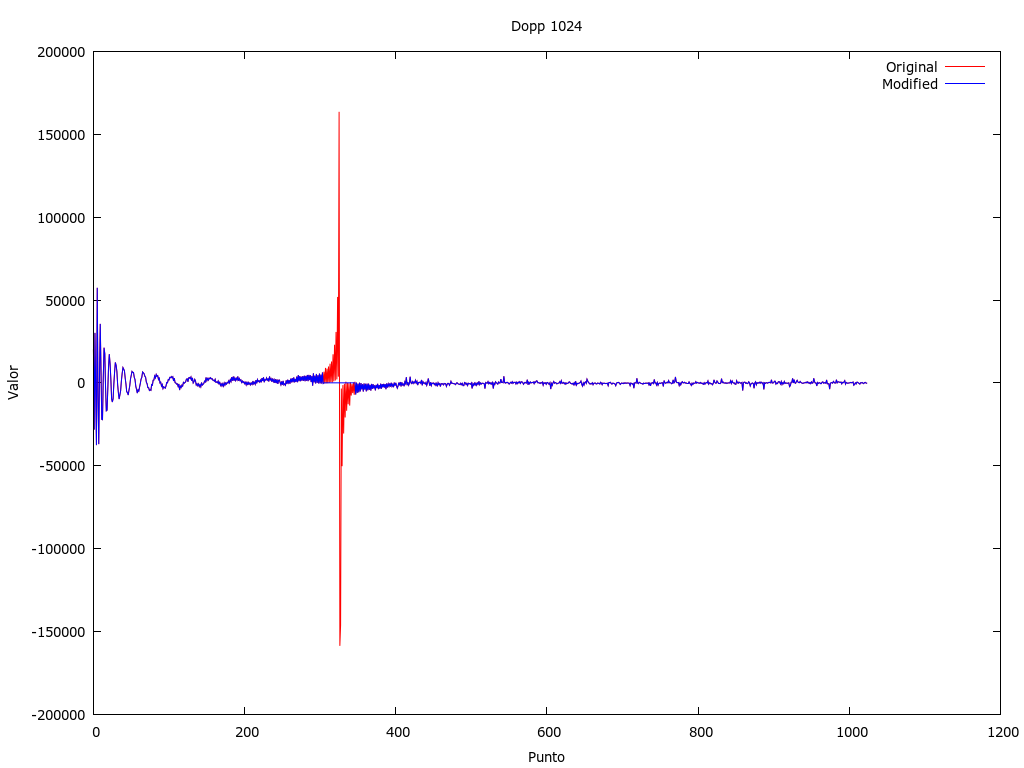
\includegraphics[width=360pt]{../matlab/dopp1024-sin100-zero-spec.png}
\end {center}
\caption{Se\~nal doppler provista por la c\'atedra, transformada, gr\'aficada
luego de aplicar ruido senoidal utilizando el multiplicador 100 (Rojo) y 
habiendo aplicado el filtro cero (azul)}
\label{fig:SinProm}
\end{figure}

Pudimos observar entonces que la se\~nal detecta frecuencias fuera del umbral y
las manda a cero. Este filtro carece de dos caracter\'isticas fundamentales
seg\'un demuestran los experimentos:

\begin{itemize}
	\item {\bf detecci\'on de ``zonas afectadas'':} Como el algoritmo no tiene en
cuenta el contexto a la hora de modificar un punto, la decisi\'on es mandar los
puntos duera del umbral al cero. Esto lleva a ``saltos'' pronunciados en la se\
~nal recuperada.

	\item {\bf elecci\'on de la correspondencia de los puntos fuera del umbral:}
El filtro decide enviar todos los elementos fuera del umbral al cero, con un
manejo de los m\'aximos y minimos globales (en el punto anterior se habla de
locales) se podr\'ia mejorar el resultado del filtro.
\end{itemize}

Sin embargo, como se aprecia en la im\'agen, los resultados son suficientemente
buenos teniendo en cuenta la simplicidad de la implementaci\'on del algoritmo.

\subsubsection{Filtro Exponencial}

Este filtro surge como una mejora del Filtro Cero. La idea que proviene de
observar los resultados provistos por el Filtro Cero est\'a relacionada con la
noci\'on de agregado de ``zona afectada'' ante la detecci\'on de un punto fuera
del umbral determinado. Como se ve a continuaci\'on, esta modificaci\'on trae
acarreada el mantenimiento de cierto grado de informaci\'on en los puntos que
decimos recuperados as\'i como de una mayor suavidad a la se\~nal recuperada.


\begin{figure}
\begin {center}
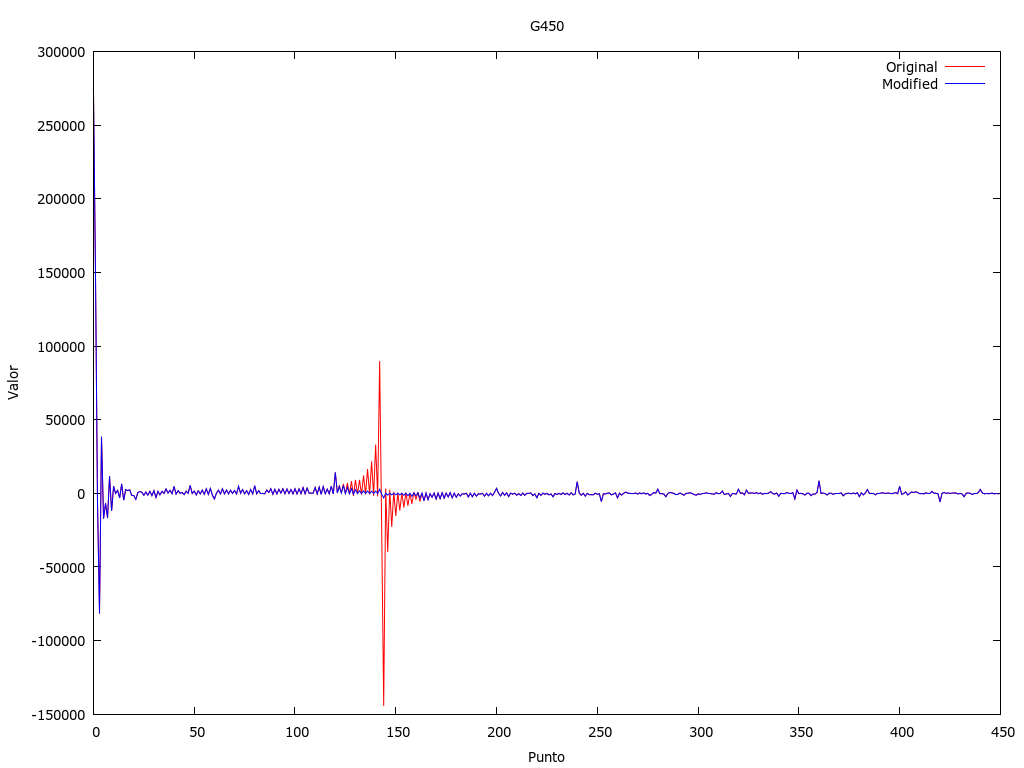
\includegraphics[width=360pt]{../matlab/g450-sin100-exp-spec.png}
\end {center}
\caption{Se\~nal g450 provista por la c\'atedra, transformada, gr\'aficada
luego de aplicar ruido senoidal utilizando el multiplicador 100 (Rojo) y 
habiendo aplicado el filtro exponencial (azul)}
\label{fig:SinProm}
\end{figure}

\begin{figure}
\begin {center}
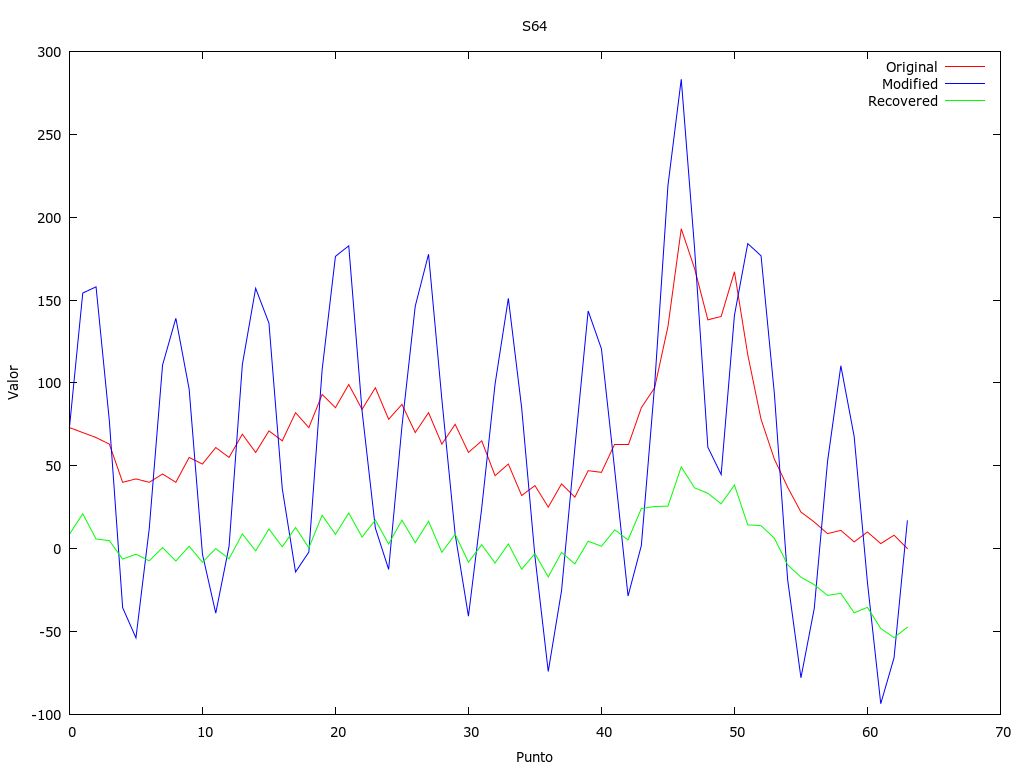
\includegraphics[width=360pt]{../matlab/s64-sin100-exp.png}
\end {center}
\caption{Se\~nal s64 provista por la c\'atedra, no transformada, gr\'aficada
luego de aplicar ruido senoidal utilizando el multiplicador 100 (Rojo) y 
habiendo aplicado el filtro promedio (azul)}
\label{fig:SinProm}
\end{figure}


\subsubsection{Filtro Promedio}

El filtro promedio, en contraposici\'on con el exponencial, toma un promedio
local a la hora de modificar elementos de la se\~nal. Esto se traduce en un
filtro poderoso que devuelve a la se\~nal un estado similar al original.

\begin{figure}
\begin {center}
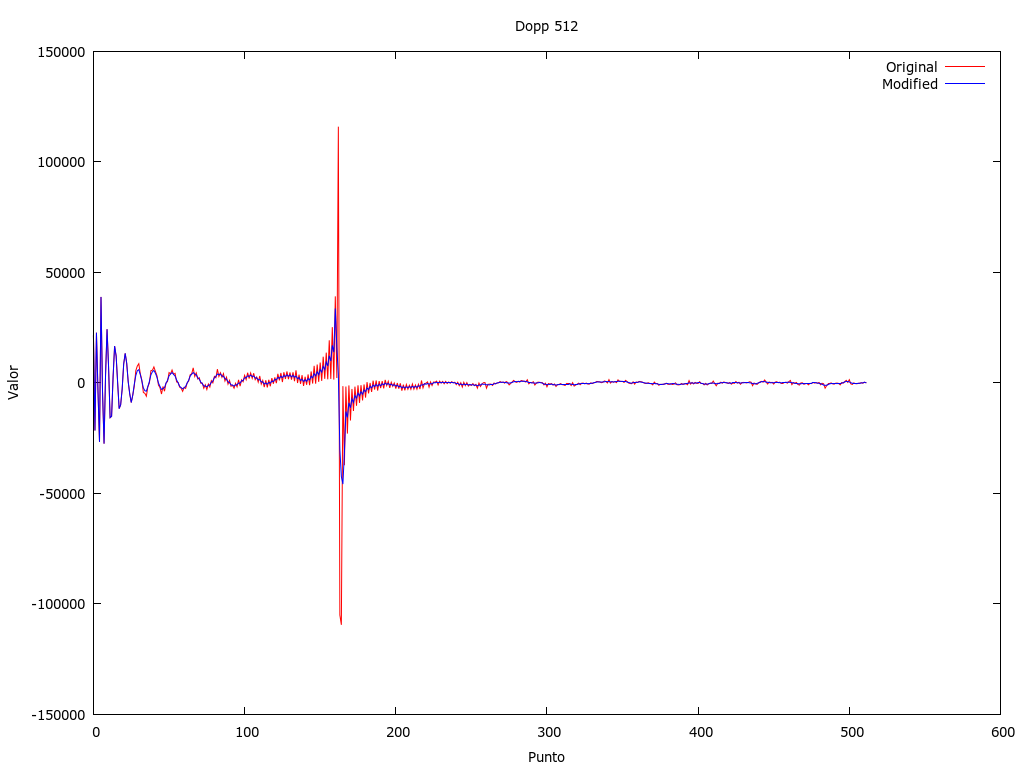
\includegraphics[width=360pt]{../matlab/dopp512-sin100-avg-spec.png}
\end {center}
\caption{Se\~nal doppler provista por la c\'atedra, transformada, gr\'aficada
luego de aplicar ruido senoidal utilizando el multiplicador 100 (Rojo) y 
habiendo aplicado el filtro promedio (azul)}
\label{fig:SinProm}
\end{figure}

\subsubsection{M\'ultiples filtros}

Otra variante utilizada fue la combinaci\'on de los filtros exponencial y
promedio. Al filtrar la se\~nal ruidosa con ambos filtros obtuvimos excelentes
resultados.

\begin{figure}
\begin {center}
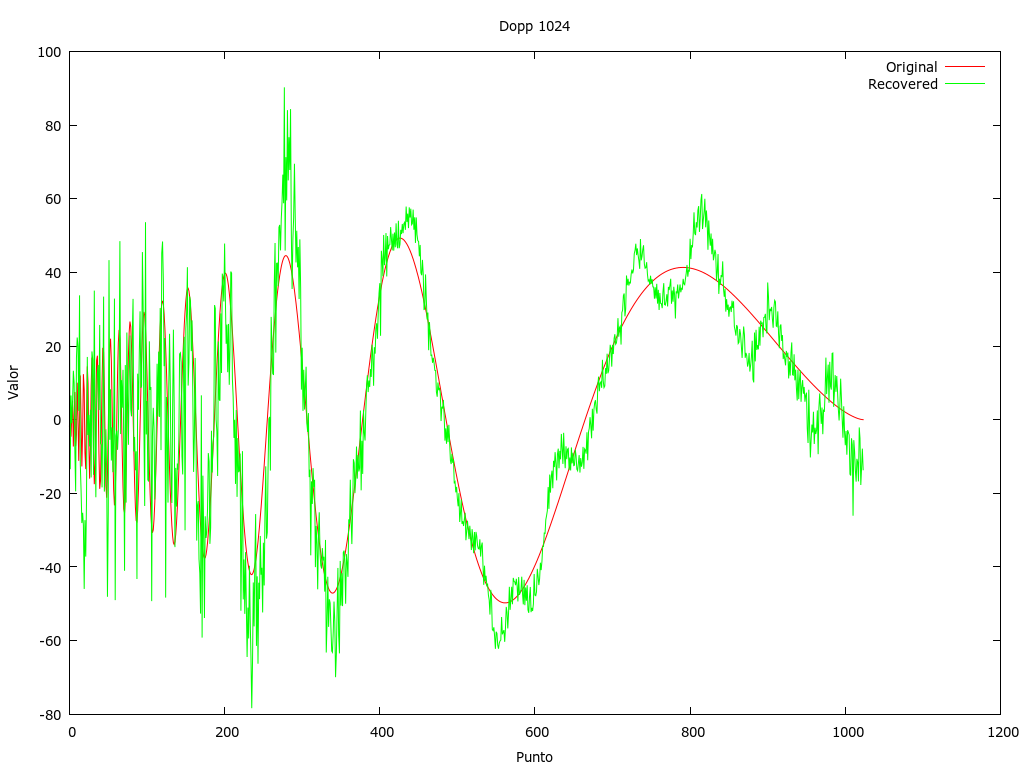
\includegraphics[width=360pt]{../matlab/dopp1024-gauss100-both.png}
\end {center}
\caption{Se\~nal doppler provista por la c\'atedra, no transformada, gr\'aficada
luego de aplicar ruido gaussiano utilizando una amplitud de 100 (Rojo) y 
habiendo aplicado los filtros promedio y exponencial (verde)}
\label{fig:SinProm}
\end{figure}

\begin{figure}
\begin {center}
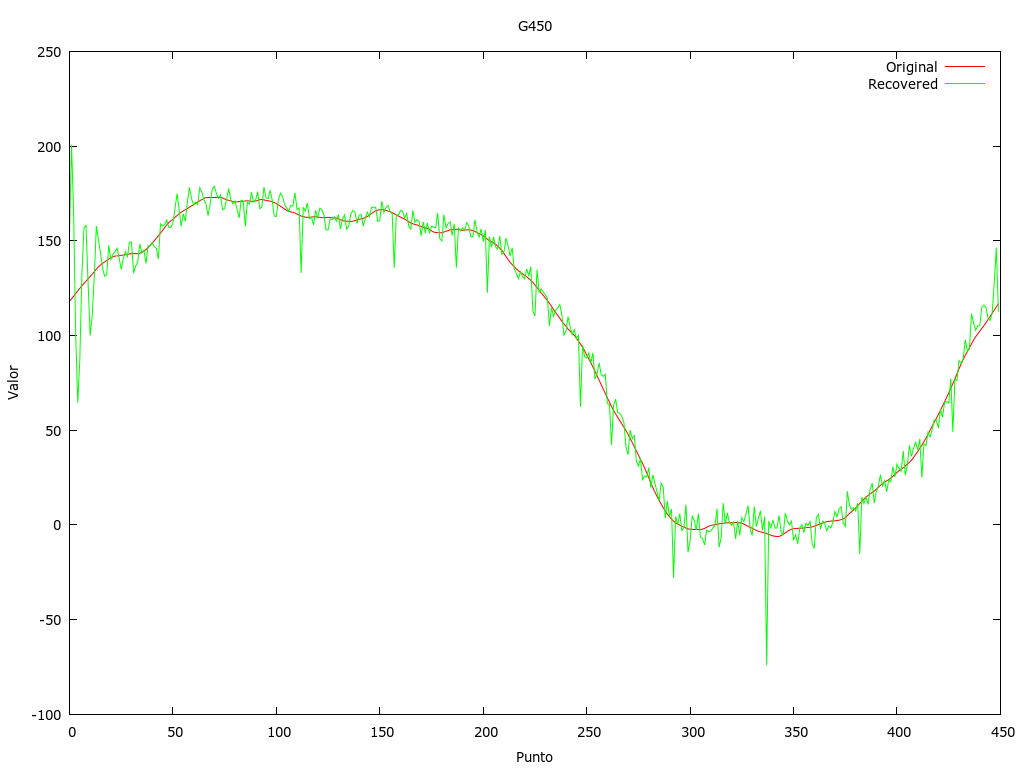
\includegraphics[width=360pt]{../matlab/g450-sin100-both.png}
\end {center}
\caption{Se\~nal g450 provista por la c\'atedra, no transformada, gr\'aficada
luego de aplicar ruido senoidal utilizando el multiplicador 100 (Rojo) y 
habiendo aplicado los filtros promedio y exponencial (verde)}
\label{fig:SinProm}
\end{figure}

\begin{figure}
\begin {center}
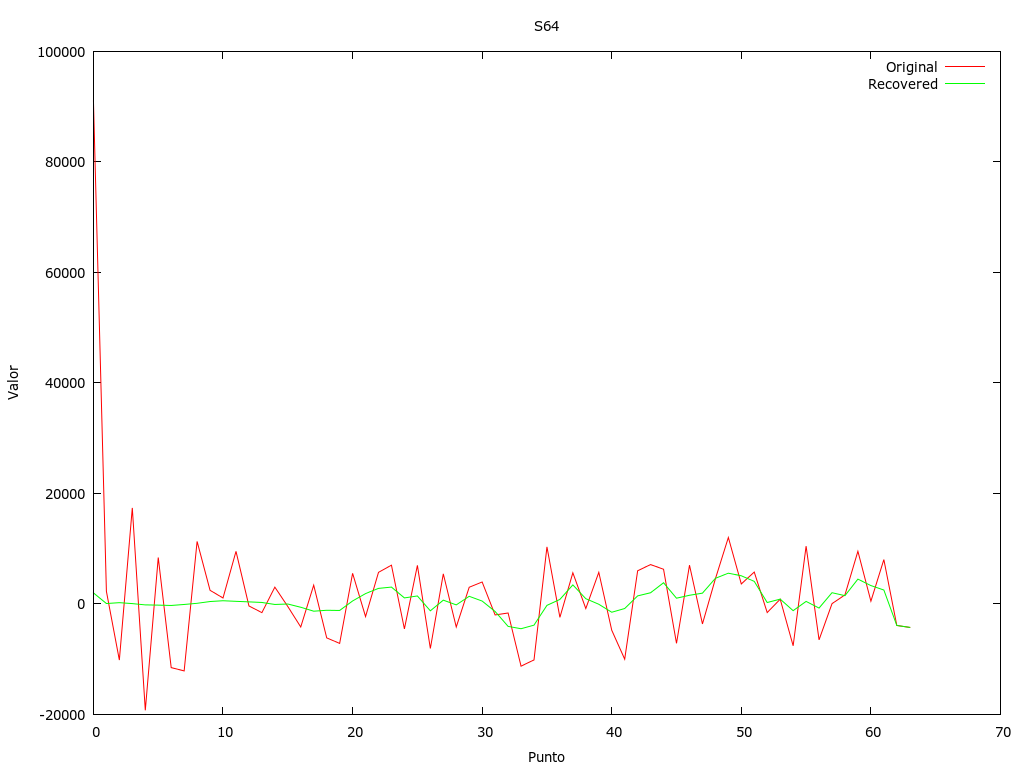
\includegraphics[width=360pt]{../matlab/s64-gauss100-both-spec.png}
\end {center}
\caption{Se\~nal s64 provista por la c\'atedra, transformada, gr\'aficada
luego de aplicar ruido gaussiano utilizando una amplitud de 100 (Rojo) y 
habiendo aplicado los filtros promedio y exponencial (verde)}
\label{fig:SinProm}
\end{figure}


\subsection{Se\~nales en dos dimensiones}

Como fue comentado, durante el desarrollo del experimento se utilizaron
im\'agenes en escala de grises. La imagen tomada como est\'andar y homenaje es 
la de Brian Kernighan.

\begin{figure}[H]
\begin {center}
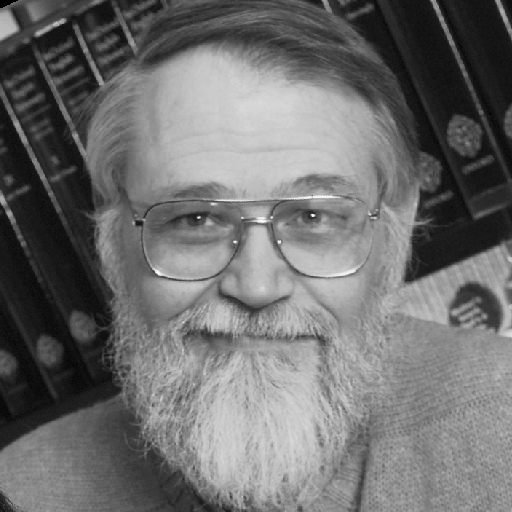
\includegraphics[width=360pt]{../datos/brian_kernighan.pgm}
\end {center}
\caption{Imagen original en escala de grises de Brian Kernighan}
\label{fig:SinProm}
\end{figure}

Habiendo mostrado las diferencias entre la implementaci\'on de los filtros en
una dimensi\'on y habiendo portado el filtrado a trav\'es de la toma de cada
fila de la im\'agen como una se\~nal de una dimensi\'on, procedemos a mostrar
los resultados obtenidos en funci\'on de los ruidos aplicados, a diferencia de
lo realizado con una dimensi\'on, donde el foco est\'a puesto en discriminar los
resultados por tipo de filtro.

\subsubsection{Ruido senoidal con multiplicador de 50}

Este ruido es controlado y es as\'i como tambi\'en los filtros pueden volver a
una imagen muy similar a la original.

\begin{figure}[H]
\begin {center}
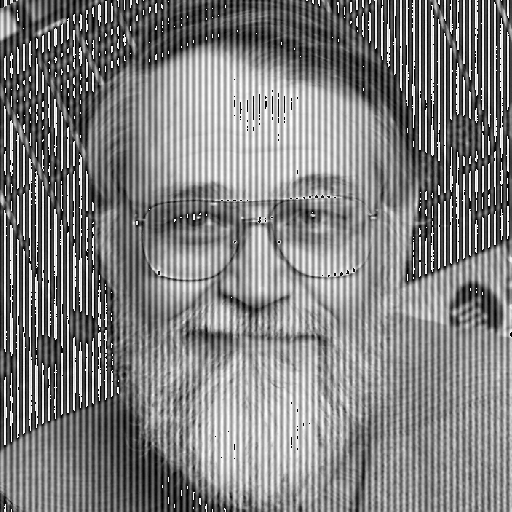
\includegraphics[width=360pt]{../matlab/kern-sin50-noisy.pgm}
\end {center}
\caption{Imagen con ruido senoidal con multiplicador de 50}
\label{fig:SinProm}
\end{figure}

\begin{figure}[H]
\begin {center}
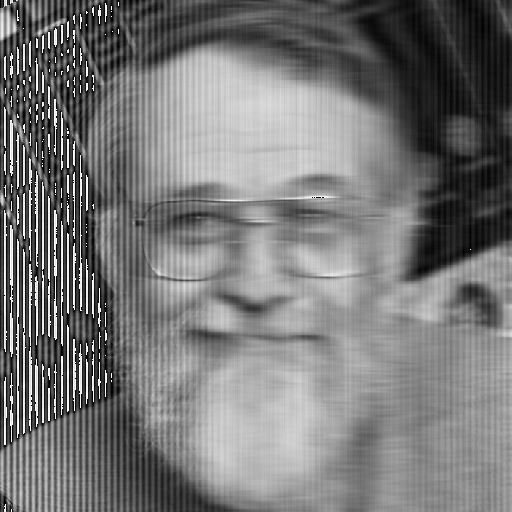
\includegraphics[width=360pt]{../matlab/kern-sin50-recovered-avg.pgm}
\end {center}
\caption{Recuperada con filtro promedio}
\label{fig:SinProm}
\end{figure}

\begin{figure}[H]
\begin {center}
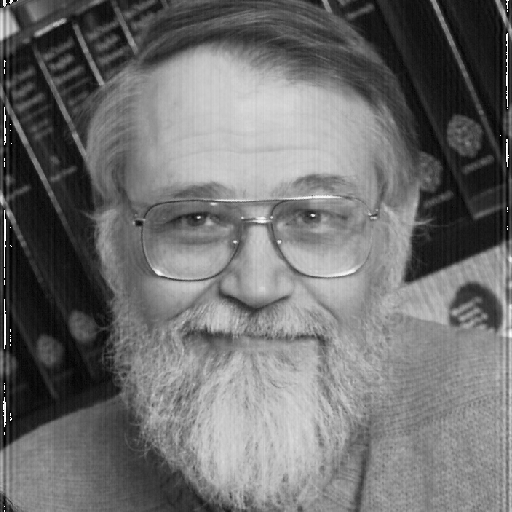
\includegraphics[width=360pt]{../matlab/kern-sin50-recovered.pgm}
\end {center}
\caption{Recuperada aplicando los 2 filtros}
\label{fig:SinProm}
\end{figure}

\subsubsection{Ruido senoidal con multiplicador de 1000}

Este ruido es controlado pero el multiplicador es muy alto, haciendo muy dificil
la recuperaci\'on de la imagen

\begin{figure}[H]
\begin {center}

\includegraphics[width=360pt]{../matlab/kern-sin1000-noisy.pgm}
\end {center}
\caption{Imagen con ruido senoidal con multiplicador de 1000}
\label{fig:SinProm}
\end{figure}

\begin{figure}[H]
\begin {center}
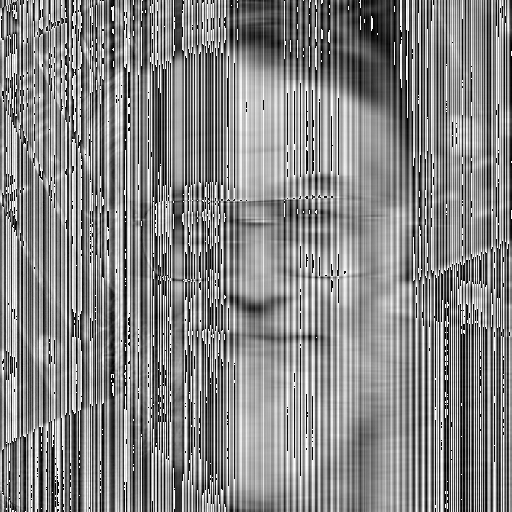
\includegraphics[width=360pt]{../matlab/kern-sin1000-recovered-avg.pgm}
\end {center}
\caption{Recuperada con filtro promedio}
\label{fig:SinProm}
\end{figure}

\begin{figure}[H]
\begin {center}
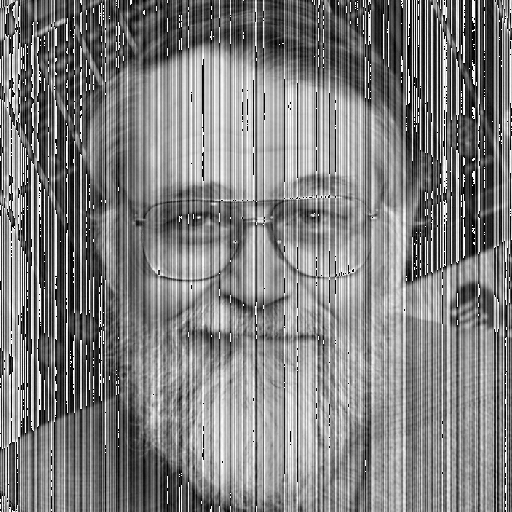
\includegraphics[width=360pt]{../matlab/kern-sin1000-recovered.pgm}
\end {center}
\caption{Recuperada aplicando los 2 filtros}
\label{fig:SinProm}
\end{figure}


\subsubsection{Ruido gaussiano con factor 100}

Este filtro fue el m\'as desafiante ya que el ruido blanco es muy d\'ificil de
capturar por su condici\'on de ``antipatron''

\begin{figure}[H]
\begin {center}
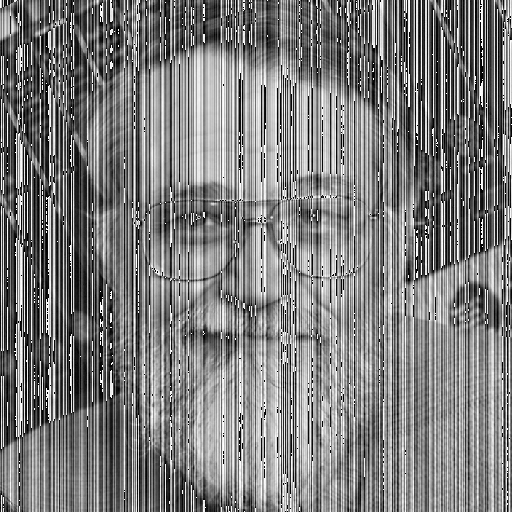
\includegraphics[width=360pt]{../matlab/kern-gauss100-noisy.pgm}
\end {center}
\caption{Imagen con ruido gaussiano con factor 1000}
\label{fig:SinProm}
\end{figure}

\begin{figure}[H]
\begin {center}
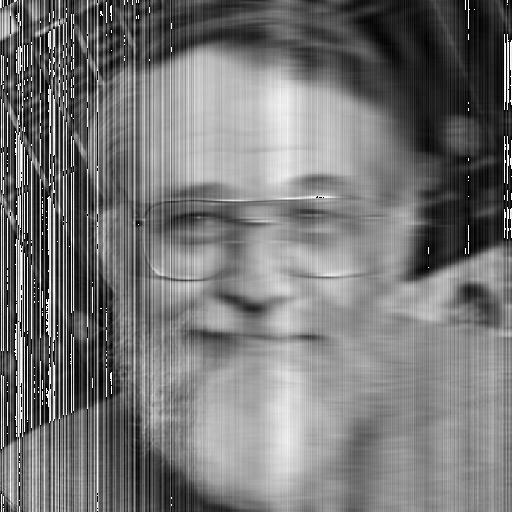
\includegraphics[width=360pt]{../matlab/kern-gauss100-recovered-avg.pgm}
\end {center}
\caption{Recuperada con filtro promedio}
\label{fig:SinProm}
\end{figure}

\begin{figure}[H]
\begin {center}
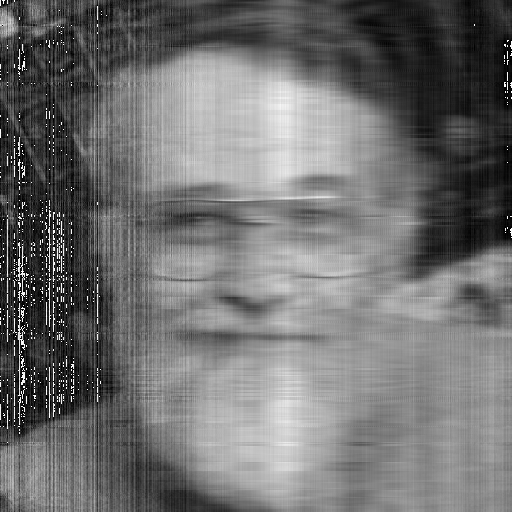
\includegraphics[width=360pt]{../matlab/kern-gauss100-recovered-both.pgm}
\end {center}
\caption{Recuperada aplicando los 2 filtros}
\label{fig:SinProm}
\end{figure}


\pagebreak


\index{Discusi\'on}
\section{Discusi\'on}

En un primer momento, el \'enfasis estuvo puesto en hacer funcionar el m\'etodo 
de Newton.
Este m\'etodo fue el primero en ser planteado e implementado debido a la
importancia recibida tanto en clase como en el material de lectura consultado.
Consecuentemente con lo esperado el m\'etodo de Newton funcion\'o exitosamente
sin la necesidad de mayores incursiones en el c\'odigo original o en las cuentas
realizadas previamente.

Luego, investigando por los otros m\'etodos de c\'alculo de ra\'ices; 
el primero que se present\'o fue la aproximaci\'on num\'erica de Newton, 
el m\'etodo de la secante. Las complejidades encontradas para el desarrollo de 
esta funci\'on fueron la facilidad con la cual el denominador tiende a cero, 
convirtiendo la cuenta en NaN (Not a Number) rapidamente. Elegimos para 
reemplazarlo el m\'etodo de Regula Falsi.

Un detalle interesante es que entre m\'as decimales se emplean, m\'as rapido 
converge el m\'etodo de Newton. Esto tiene sentido debido a que las 
aproximaciones num\'ericas son cada vez mejores. Tambi\'en se observa que para 
valores de precision muy bajos (menos de 14 decimales binarios en promedio), 
Newton directamente diverge. 
Este fenomeno se debe a que la precisi\'on del epsilon elegido 
($\epsilon = 10^{-4}$) es apenas mayor que $2^{-14}$. 
Esto produce que queden pocos bits para la que ser\'ia parte entera dentro de 
la mantisa. Como esos bits se tienen que compartir entre parte entera y parte 
decimal, no se tienen exactamente 14 bits para los decimales, sino que a medida 
que se va a agrandando el n\'umero, la densidad de los reales representables 
disminuye dr\'asticamente.

Fue de inter\'es trazar las curvas de aproximaci\'on de las variables. 
Esto es de alta relevancia ya que se puede ver realmente el impacto que se tiene
al utilizar mayor cantidad de d\'igitos. Lo m\'as notable fue visuzalizar la 
aproximaci\'on asint\'otica a los valores ``verdaderos'' de las variables, 
y como las ganancias marginales a partir de, en promedio, 22 decimales, 
se vuelven despreciables. Nuestra hip\'otesis es que con esa cantidad de 
d\'igitos, la mantisa puede ser suficientemente bien ajustada a tal punto que puede 
ser representada bien la parte entera y la parte decimal minimice los errores de 
operaci\'on. Por ejemplo, en el caso 1, como $\beta = 9$, se necesitan al menos 
5 bits para representar la parte entera. Luego, todos los restantes seran usados 
para decimales. Si hubiera 15 bits en total, quedar\'ian 10 bits para la parte 
decimal. $2^{-10}<10{-4}<2^{-9}$, luego la parte decimal, va a tener una
precisi\'on cercana a $\frac{1}{1000}$, en caso promedio. 
Sin embargo no alcanza a converger a los valores originales que generaron los 
datos por la acumulacion de errores en, por ejemplo, las funciones
de sumatoria, logaritmos y potenciaci\'on. Esta \'ultima es especialmente 
sensible a los errores en el exponente, y cuando se la procesa de forma 
acumulada (como en una sumatoria), se puede llegar a arrastrar un error
considerable. Como la funci\'on que estima
$\beta$ utiliza sucesivas sumatorias y potencia, podemos ver que ese es un punto 
importante a la hora de intentar minimizar el error de la estimaci\'on.

Debido a discrepancias de convergencia en los casos 1 y 2 utilizando el m\'etodo
de Regla falsa, se procedi\'o a buscar una mejora en este que nos permita una mejor
tasa de convergencia y un ajuste en los valores. Esto fue logrado mediante la
implementaci\'on del algoritmo de Illinois. Gracias a esta mejora se alcanzaron 
mejores curvas de valores.

Como podemos ver en las figuras \ref{fig:FitCaso4Newton} y \ref{fig:Fit4Y7Newton}, la aproximaci\'on que obtenemos de $\beta$ se ajusta bastante
a los datos a\'un con poca precisi\'on cuando utilizamos el m\'etodo de Newton. En la figura 4 podemos
observar que a partir de 22 bits de precisi\'on el valor de $\beta$ se acerca lo suficiente al valor
al cual converge.

En las figuras \ref{fig:FitCaso3RegulaFalsi} y \ref{fig:FitCaso4RegulaFalsi} observamos que, utilizando el m\'etodo de Regula Falsi (en su versi\'on Illinois)
con 15 bits de precisi\'on el valor de $\beta$ no es lo suficientemente adecuado como para que la curva
se ajuste a los datos. A partir de 17 bits de precisi\'on, en cambio, ya empieza a acercarse m\'as curva
a lo que vale realmente de acuerdo a lo que podemos observar comparandola con los datos de entrada.

En la figura \ref{fig:FitCaso4Y7RegulaFalsi} observamos que a partir de 22 d\'igitos de precisi\'on binaria el valor de $\beta$ empieza
a acercarse al valor al cual converge, al igual que con el m\'etodo de Newton.

En la figura \ref{fig:Newton-Eps-Caso4} graficamos la cantidad de iteraciones y el valor de $\beta$ en funci\'on del valor de $\epsilon$
que utilizamos. Podemos observar que, con 21 bits de presici\'on, a partir de un $\epsilon$ de $10^{-5}$ el m\'etodo
empieza a cortar por cantidad de iteraciones y $\beta$ empieza a converger correctamente.

Con 50 bits de precisi\'on, en cambio, $\beta$ converge a partir de un $\epsilon$ de $10^{-3}$ y corta siempre por 
el $\epsilon$ en lugar de por cantidad de iteraciones. Esto se debe a que al haber m\'as precisi\'on el m\'etodo converge m\'as
r\'apido y a un valor m\'as exacto.

Con Regula Falsi podemos observar un comportamiento similar en lo que respecta a cantidad de iteraciones, aunque para asegurar
la convergencia debemos tener un valor de $\epsilon$ m\'as chico. Esto se debe a que el m\'etodo no es tan eficiente como el
m\'etodo de Newton.


\pagebreak

\section{Conclusiones}

La primer conclusi\'on que pudimos sacar de este TP fue que el filtro que apliquemos para detecci\'on y correci\'on
de ruido siempre va a depender del tipo de ruido que querramos eliminar de la se\~nal.

Los ruidos que estudiamos fueron ruidos gaussianos y ruidos senodales. En ambos casos pudimos comparar los filtros
exponenciales y promediadores que desarrollamos contra las sen\~nales originales, y alguno de estos o la combinaci\'on de los dos,
resultaron razonablemente efectivos a la hora de restaurar la mayor integridad posible.

En se\~nales 1D los filtros que aplicamos reconstruyeron se\~nales que se parecieron mucho m\'as a la se\~nal
original que la se\~nal con ruido aunque en muchos casos la diferencia era notable. Se puede percibir esto en las zonas
de alta frecuencia de la imagen. Se pudo notar ahi que el filtro promediador, incluso con coeficientes que preservaran
bastante las se\~nales originales en las frecuencia no alteradas por ruido, que estos peque\~nos cambios alcanzaban a
variar muchisimo la se\~nal reconstruida. Esto nos dejo bien claro que hay que tener cuidado a la hora de hacer alteraciones
en la base de los cosenos, no es para intuito el resultado que produce una perturbaci\'on en la reconstruccion de las se\~nales.

En se\~nales 2D, en cambio, ya que trabajabamos con im\'agenes, pudimos observar que la imagen con ruido en muchos
casos no se distingu\'ia (es decir, no se pod\'ia reconocer la imagen comparandola con la original), aunque despu\'es
de aplicar los filtros se reconoce una imagen bastante fiel a la original en comparaci\'on con la imagen ruidosa.
Es importante saber los casos de uso de las funciones para definir el rango de calidad \textit{aceptable}. No es lo mismo
la precision necesaria para identificar si hay, o no, una cara en la imagen que para un sistema de reconocimiento \'optico
de caracteres. Esto es clave para poder ver si se justifica aplicar filtros como promediador, donde se pierden un poco de detalles como suavizado
pero se gana en velocidad de identificaci\'on humana.

Lamentablemente, nos hubiera gustado contar con un tiempo adicional para intentar los filtros por bloques, como sugeria el ejercicio
opcional. \textit{A priori}, nos damos cuenta que son excelentes herramientas para mejorar el tiempo de ejecuci\'on
de las transformaciones, ya que el crecimiento cuadr\'atico y c\'ubico de la resoluci\'on de sistemas se not\'o claramente
Sin estas optimizaciones, seria imposible realizar sistemas de filtros por software en tiempo real, eliminando un campo de 
aplicaci\'on gigantesco. Sin embargo, sabemos que productos comerciales con estas caracteristicas existen, por lo que
seria interesante conocer los detalles de implementaci\'on para poder reconocer donde estan los cuellos de botella y como
eliminarlos.

En resumen, con este trabajo pudimos comprender un m\'inimo de la importancia de la transformacion de Fourier y similares,
un \'area que ha sido crucial para el desarrollo de las telecomunicaciones alrededor del mundo. Nos ha servido para plantear
el problema desde otro aspecto, como un ``simple'' cambio de base puede revelarnos mucha mas informaci\'on de la que 
consideramos existente en una se\~nal. 


\pagebreak

\section{Apendice A, Codigo del TP}
\begin{lstlisting}

#include <algorithm>
#include <cmath>
#include <cstdio>
#include <iomanip>
#include <iostream>
#include <queue>
#include <set>
#include <sstream>
#include <string>
#include <vector>

#include "TFloat.h"
#include <math.h>

#ifdef __gnu_linux__
#include "timetools.h"
#endif
using namespace std;

vector < TFloat > valores;

int n, t;
double epsilon = 1.e-4;
int maximoIteraciones = 10;
TFloat pot(TFloat base, TFloat exp)
{
    double result = pow(base.dbl(), exp.dbl());
    return TFloat(result, t);
}

TFloat log(TFloat d)
{
    double result = log(d.dbl());
    return TFloat(result, t);
}

TFloat M(TFloat s)
{
    TFloat res = TFloat(0., t);
    for (int i = 0; i < n; i++)
	res = res + pot(valores[i], s);
    res = res / TFloat(n, t);
    return res;
}

TFloat MSombrero(TFloat s)
{
    TFloat res = TFloat(0., t);
    for (int i = 0; i < n; i++)
	res = res + pot(valores[i], s) * log(valores[i]);
    res = res / TFloat(n, t);
    return res;
}

TFloat MPrima(TFloat s)
{
    // / Resulta ser que Mprima es igual a Msombrero
    return MSombrero(s);
}

TFloat MSombreroPrima(TFloat s)
{
    TFloat res = TFloat(0., t);
    for (int i = 0; i < n; i++)
	res = res + pot(valores[i], s) * log(valores[i]) * log(valores[i]);
    res = res / TFloat(n, t);
    return res;
}

TFloat R(TFloat s)
{
    return MSombrero(s) / M(s);
}

TFloat RPrima(TFloat s)
{
    return (MSombreroPrima(s) * M(s) -
	    MSombrero(s) * MPrima(s)) / (M(s) * M(s));
}

TFloat Lambda(TFloat beta)
{
    vector < TFloat > logvals(n);
    vector < TFloat > xbeta(n);
    TFloat sumalogvals(0.0, t);
    TFloat sumaxbeta(0.0, t);
    TFloat sumalogxbeta(0.0, t);
    for (int i = 0; i < n; i++)
      {
	  logvals[i] = log(valores[i]);
	  xbeta[i] = pot(valores[i], beta);
      }
    for (int i = 0; i < n; i++)
      {
	  sumalogvals = sumalogvals + logvals[i];
	  sumaxbeta = sumaxbeta + xbeta[i];
	  sumalogxbeta = sumalogxbeta + logvals[i] * xbeta[i];
      }
    TFloat lambda =
	pot(beta *
	    (((sumalogxbeta) / (sumaxbeta)) -
	     ((sumalogvals) / (TFloat(n, t)))),
	    TFloat(-1, t));
    return lambda;

}

TFloat Sigma(TFloat beta, TFloat lambda)
{
    TFloat sigma;
    TFloat xbetasuma(0.0, t);

    for (int i = 0; i < n; i++)
      {
	  xbetasuma = xbetasuma + pot(valores[i], beta);
      }
    sigma =
	pot((xbetasuma / (TFloat(n, t) * lambda)),
	    (TFloat(1.0, t) / beta));

    return sigma;
}

TFloat f(TFloat beta)
{
    TFloat Mbeta = M(beta);
    TFloat res =
	M(beta * 2) / (Mbeta * Mbeta) - beta * (R(beta) - R(0)) - 1.;
    return res;
}


TFloat fprima(TFloat beta)
{

    /** Mprima(beta*2)*2 = Derivada de M(beta*2)
     *  M(beta)*Mprima(beta)*2 = Derivada de M(beta)*M(beta) o M(beta)^2
     *  Derivada de M(beta*2)/M(beta)^2 =
     *      (Mprima(beta*2)*M(beta)*M(beta)*2 - 
		M(beta*2)*M(beta)*Mprima(beta)*2)/(M(beta)*M(beta)*M(beta)*M(beta))
     *  Derivada de beta * (R(beta) - R(0)) =
     *      beta * (Rprima(beta)) + R(beta)-R(0) 
     */

    TFloat Mbeta = M(beta);
    TFloat Mbeta2 = Mbeta * Mbeta;
    // Aca podemos simplificar varios terminos sacando factores comunes
    return (TFloat(2, t)) * (MPrima(beta * 2) * Mbeta -
			     M(beta * 2) * MPrima(beta)) / (Mbeta *
							    Mbeta2) -
	(beta * RPrima(beta) + R(beta) - R(0));
}


TFloat newton(TFloat beta, TFloat beta2, int &iteraciones)
{
    iteraciones = 0;

    while (iteraciones < maximoIteraciones
	   && abs(beta.dbl() - beta2.dbl()) > epsilon)
      {
	  iteraciones++;
	  beta2 = beta;
	  beta = beta - f(beta) / fprima(beta);
      }
    return beta;
}

TFloat illinois(TFloat beta, TFloat beta2, int &iteraciones)
{
    iteraciones = 0;
    TFloat beta3;
    TFloat fbeta = f(beta);
    TFloat fbeta2 = f(beta2);
    for (int i = 0; i < 10; i++)
	if (fbeta.dbl() > 0)
	  {
	      beta = beta / 2.;
	      fbeta = f(beta);
	  }
    for (int i = 0; i < 10; i++)
	if (fbeta2.dbl() < 0)
	  {
	      beta2 = beta2 * 2;
	      fbeta2 = f(beta2);
	  }
    if (fbeta.dbl() * fbeta2.dbl() > 0)
      {
	  cerr << setprecision(15);
	  cerr << "==================fruta follows===================\n";
	  cerr << beta.dbl() << ": " << fbeta.dbl() << "   " << beta2.
	      dbl() << ": " << fbeta2.dbl() << endl;
      }
    int side = -1;
    while (iteraciones < maximoIteraciones
	   && fabs(beta.dbl() - beta2.dbl()) > epsilon)
      {
	  iteraciones++;
	  beta3 = (fbeta * beta2 - fbeta2 * beta) / (fbeta - fbeta2);
	  TFloat fbeta3 = f(beta3);
	  if (fbeta2.dbl() * fbeta3.dbl() > 0)
	    {
		beta2 = beta3;
		fbeta2 = fbeta3;
		if (side == -1)
		    fbeta = fbeta / 2;
		side = -1;
	    }
	  else if (fbeta.dbl() * fbeta3.dbl() > 0)
	    {
		beta = beta3;
		fbeta = fbeta3;
		if (side == 1)
		    fbeta2 = fbeta2 / 2;
		side = 1;
	    }
      }
    cerr << abs(beta2.dbl() - beta.dbl()) << " " << iteraciones << endl;
    return beta3;
}

void uso()
{
    cout <<
	"\"./MN\" precision = 52, iteraciones maximas = 10, Beta entre 0.0 y 10.0"
	<< endl;
    cout <<
	"\"./MN <t>\" precision = t, iteraciones maximas = 10, Beta entre 0.0 y 10.0"
	<< endl;
    cout <<
	"\"./MN <t> <n> <b1> <b2> <m> \" precision = t, iteraciones maximas= n, Beta entre b1 y b2, <m> metodo (0 Newton - 1 RegulaFalsi)"
	<< endl;
    cout <<
	"\"./MN <t> <n> <b1> <b2> <m> <e> \" precision = t, iteraciones maximas= n, Beta entre b1 y b2, <m> metodo (0 Newton - 1 RegulaFalsi), epsilon =<e>"
	<< endl;
}

int main(int argc, char *argv[])
{
    TFloat beta = TFloat(10., 52);
    TFloat beta2 = TFloat(1., 52);
    int metodo = 0;		// 0 Newton 1 RegulaFalsi
    switch (argc)
      {
	case 1:
	    t = 52;
	    break;
	case 2:
	    t = atoi(argv[1]);
	    break;
	case 7:
	    epsilon = atof(argv[6]);
	case 6:
	    metodo = atoi(argv[5]);
	case 5:
	    t = atoi(argv[1]);
	    maximoIteraciones = atoi(argv[2]);
	    beta = TFloat(atof(argv[3]), t);
	    beta2 = TFloat(atof(argv[4]), t);
	    break;
	default:
	    uso();
	    return 1;
	    break;
      }
    cin >> n;
    valores.resize(n);
    double db;
    for (int i = 0; i < n; i++)
      {
	  cin >> db;

	  valores[i] = TFloat(db, t);
      }

    int iteraciones = 0;
    TFloat outBeta;
    TFloat outLambda;
    TFloat outSigma;

    cout << setprecision(15);

#ifdef __gnu_linux__
    timespec startTime;
    timespec endTime;

    clock_gettime(CLOCK_PROCESS_CPUTIME_ID, &startTime);
#endif

    if (metodo == 0)
      {
	  outBeta = newton(beta, beta2, iteraciones);
      }
    else if (metodo == 1)
      {
	  outBeta = illinois(beta, beta2, iteraciones);
      }

    outLambda = Lambda(outBeta);
    outSigma = Sigma(outBeta, outLambda);

#ifdef __gnu_linux__
    clock_gettime(CLOCK_PROCESS_CPUTIME_ID, &endTime);
    const timespec delta = diff(startTime, endTime);
#endif
    cout << outBeta.dbl() << " " << outLambda.dbl() << " " << outSigma.
	dbl() << " " << iteraciones;
#ifdef __gnu_linux__
    cout << " " << (delta.tv_sec * 1000 * 1000 * 1000 +
		    delta.tv_nsec) / (1000 * 1000);
#endif
    cout << endl;
    return 0;
}
\end{lstlisting}


\pagebreak

\section{Referencias}

\begin{itemize}
  \item \nocite {Burden} Burden, Richard; Faires, Douglas. An\'alisis num\'erico. Brooks Cole, 2011.
  \item \nocite {MN} Clases de M\'etodos Num\'ericos. Departamento de Computaci\'on, UBA. Primer Cuatrimestre de 2013.
\end{itemize}



\end{document}
